\documentclass[twoside,twocolumn]{article}

\usepackage{blindtext} 
\usepackage{graphicx}
\usepackage[sc]{mathpazo} 
\usepackage[T1]{fontenc} 
\linespread{1.05} 
\usepackage{microtype} 


\usepackage[english]{babel} 


\usepackage[hmarginratio=1:1,top=32mm,columnsep=20pt]{geometry} 
\usepackage[hang, small,labelfont=bf,up,textfont=it,up]{caption} 
\usepackage{booktabs} 


\usepackage{lettrine} 


\usepackage{enumitem} 
\setlist[itemize]{noitemsep} 


\usepackage{abstract} 
\renewcommand{\abstractnamefont}{\normalfont\bfseries} 
\renewcommand{\abstracttextfont}{\normalfont\small\itshape} 


\usepackage{titlesec} 
\renewcommand\thesection{\Roman{section}} % 
\renewcommand\thesubsection{\roman{subsection}} 
\titleformat{\section}[block]{\large\scshape\centering}{\thesection.}{1em}{} 
\titleformat{\subsection}[block]{\large}{\thesubsection.}{1em}{} 


\usepackage{fancyhdr} 
\pagestyle{fancy} 
\fancyhead{} 
\fancyfoot{} 
\fancyhead[C]{API testing frameworks $\bullet$ May 2023 $\bullet$ } 
\fancyfoot[RO,LE]{\thepage} 


\usepackage{titling} 


\usepackage{hyperref} 


%----------------------------------------------------------------------------------------
%	TILULOS
%----------------------------------------------------------------------------------------


\setlength{\droptitle}{-4\baselineskip} 
\pretitle{\begin{center}\Huge\bfseries} 
\posttitle{\end{center}}
\title{API testing frameworks} 
\author{Erick Mamani Lima, Helbert Andres Condori Loayza \\
Diego Andre Aranda Reyes, Jhonny Rivera Mendoza. }
\date{\today} 
\renewcommand{\maketitlehookd}{
\begin{abstract}
\noindent 
API testing frameworks are tool sets and libraries that facilitate the creation, execution, and management of API tests. They provide a framework and specific functionalities for automated testing, response validation, load testing, and detailed reporting. In this article, Postman and Swagger, two popular frameworks, are compared. They offer advanced capabilities for API testing and documentation, such as test automation, team collaboration, and interactive documentation generation. The article explores usability, flexibility, automation, reporting, and collaboration in both frameworks, providing practical examples to illustrate their usage.
\end{abstract}
\begin{abstract}
\noindent 
Los frameworks de API son conjuntos de herramientas y bibliotecas que facilitan la creación, ejecución y gestión de pruebas de API. Proporcionan un marco y funcionalidades específicas para pruebas automatizadas, validación de respuestas, pruebas de carga e informes detallados. En este artículo, se comparan Postman y Swagger, dos frameworks populares. Ofrecen capacidades avanzadas para pruebas y documentación de API, como automatización de pruebas, colaboración en equipo y generación de documentación interactiva. El artículo explora la usabilidad, la flexibilidad, la automatización, la generación de informes y proporciona ejemplos prácticos para ilustrar su uso.
\end{abstract}
}

%----------------------------------------------------------------------------------------
\begin{document}
% Print the title
\maketitle
%----------------------------------------------------------------------------------------
%	INTRODUCCION
%----------------------------------------------------------------------------------------

\section{Introduction}
\lettrine[lines=3]{I}n the era of digital transformation and agile software development, APIs (Application Programming Interfaces) play a crucial role in connecting applications, sharing data, and fostering integration between systems.


API testing is a set of quality assurance actions that involve sending calls to the API, retrieving output, and validating the system's response against defined input parameters, including data accuracy, data format, HTTP status codes, and error codes (altexsoft, 2022).


Within the realm of API testing, it is common to focus on APIs produced by the internal development team. These APIs are specifically created for use within the organization's environment and context. 

The goal of API testing is to enhance the overall quality, performance, and usability of the applications that rely on these APIs, fostering a seamless user experience and enabling successful interactions between different software components. 

In this article, we will explore a comparison between two of the most popular frameworks used for API testing: Postman and Swagger. These tools have gained recognition in the industry for their ability to simplify and automate the API testing process, yet each offers unique approaches and features.

Throughout this comparison, we will examine key aspects such as ease of use, flexibility, automation capabilities, reporting generation, and team collaboration. By the end of this article, you will have a clear understanding of the advantages and disadvantages of Postman and Swagger, enabling you to make an informed decision on which one best fits your specific needs in the realm of API testing.
%----------------------------------------------------------------------------------------
%	Objetivos
%----------------------------------------------------------------------------------------

%----------------------------------------------------------------------------------------
%	DESARROLLO
%----------------------------------------------------------------------------------------

\section{Body}
\subsection{Swagger}
\\ \\
Swagger is an API testing tool that allows users to start their functional, security, and performance testing right from the Open API Specifications. Swagger tooling and Ready API platform make it easy to quickly create, manage, and execute API tests in the pipeline.
That's why Swagger has quickly become the most popular technology for API documentations. Rather, it has become the most popular technology for the most frequently used REST APIs. Swagger was developed by Reverb, but is now characterized by its neutrality as open source under the Linux Foundation's Open API Initiative. Over time, Swagger has been renamed to the OpenAPI specification, although it is still unofficially known as Swagger.
\\ \\

 \textbf{ What it is used for?}
\\ \\
For API development, it is essential to have a tidy and understandable documentation, because only then can the developers' interfaces be used. This is even more important for public APIs: without documentation, they are useless to the community, cannot be disseminated and do not bring success.

Right now, Swagger is the best choice for documenting REST APIs, because it can represent almost all web services and information around the interface. It grows at the same pace as the system and documents changes automatically. Operation is trouble-free, because Swagger deposits the REST API documentation directly into the REST API code.
\\ \\


 \textbf{ Swagger: the advantages of maintaining order}
\\ \\
Its advantages are such that Swagger can be defined as the standard application par excellence for describing interfaces in RESTful APIs. Like many other open source applications, Swagger enjoys wide distribution and thus compatibility with many tools. The Swagger guild is made up of technology giants such as Microsoft, IBM and Google, which means that the OpenAPI specification has unconditional support, even though there are alternatives such as Restful API Modelling Language (RAML). This is also based on YAML and develops even more complex definitions than Swagger, but even its creator (Mulesoft) has joined the OpenAPI Initiative.

A small disadvantage of Swagger is the comprehensibility and readability of the documentation. Although Swagger offers a relatively well-crafted format, it takes some time to become familiar with it. Proof that it can be simpler is the Blueprint API, with its Markdown syntax.
\\ \\


 \textbf{Swagger Inspector }
\\ \\
Swagger Inspector is a tool that facilitates quick and easy API testing and documentation. It provides an intuitive interface that allows you to send requests to an API and receive the corresponding responses, which helps you validate and analyze the behavior of the API.
\\ \\


 \textbf{benefits of Swagger Inspector}
\\ \\
API testing without complex configuration: Swagger Inspector simplifies the API testing process by allowing you to send requests quickly and easily. There is no need to set up a complex environment or write additional code.

Automatic API documentation: As requests are sent and responses are received in Swagger Inspector, the tool automatically generates basic API documentation in Swagger format. This makes it easy to document the API and share information with other developers.

Response validation and analysis: Swagger Inspector clearly displays the responses obtained from the API, allowing you to validate the accuracy and structure of the returned data. It also provides analysis capabilities to inspect headers, response body and other relevant details.
\\ \\
\textbf{example in Swagger }
\begin{center}
	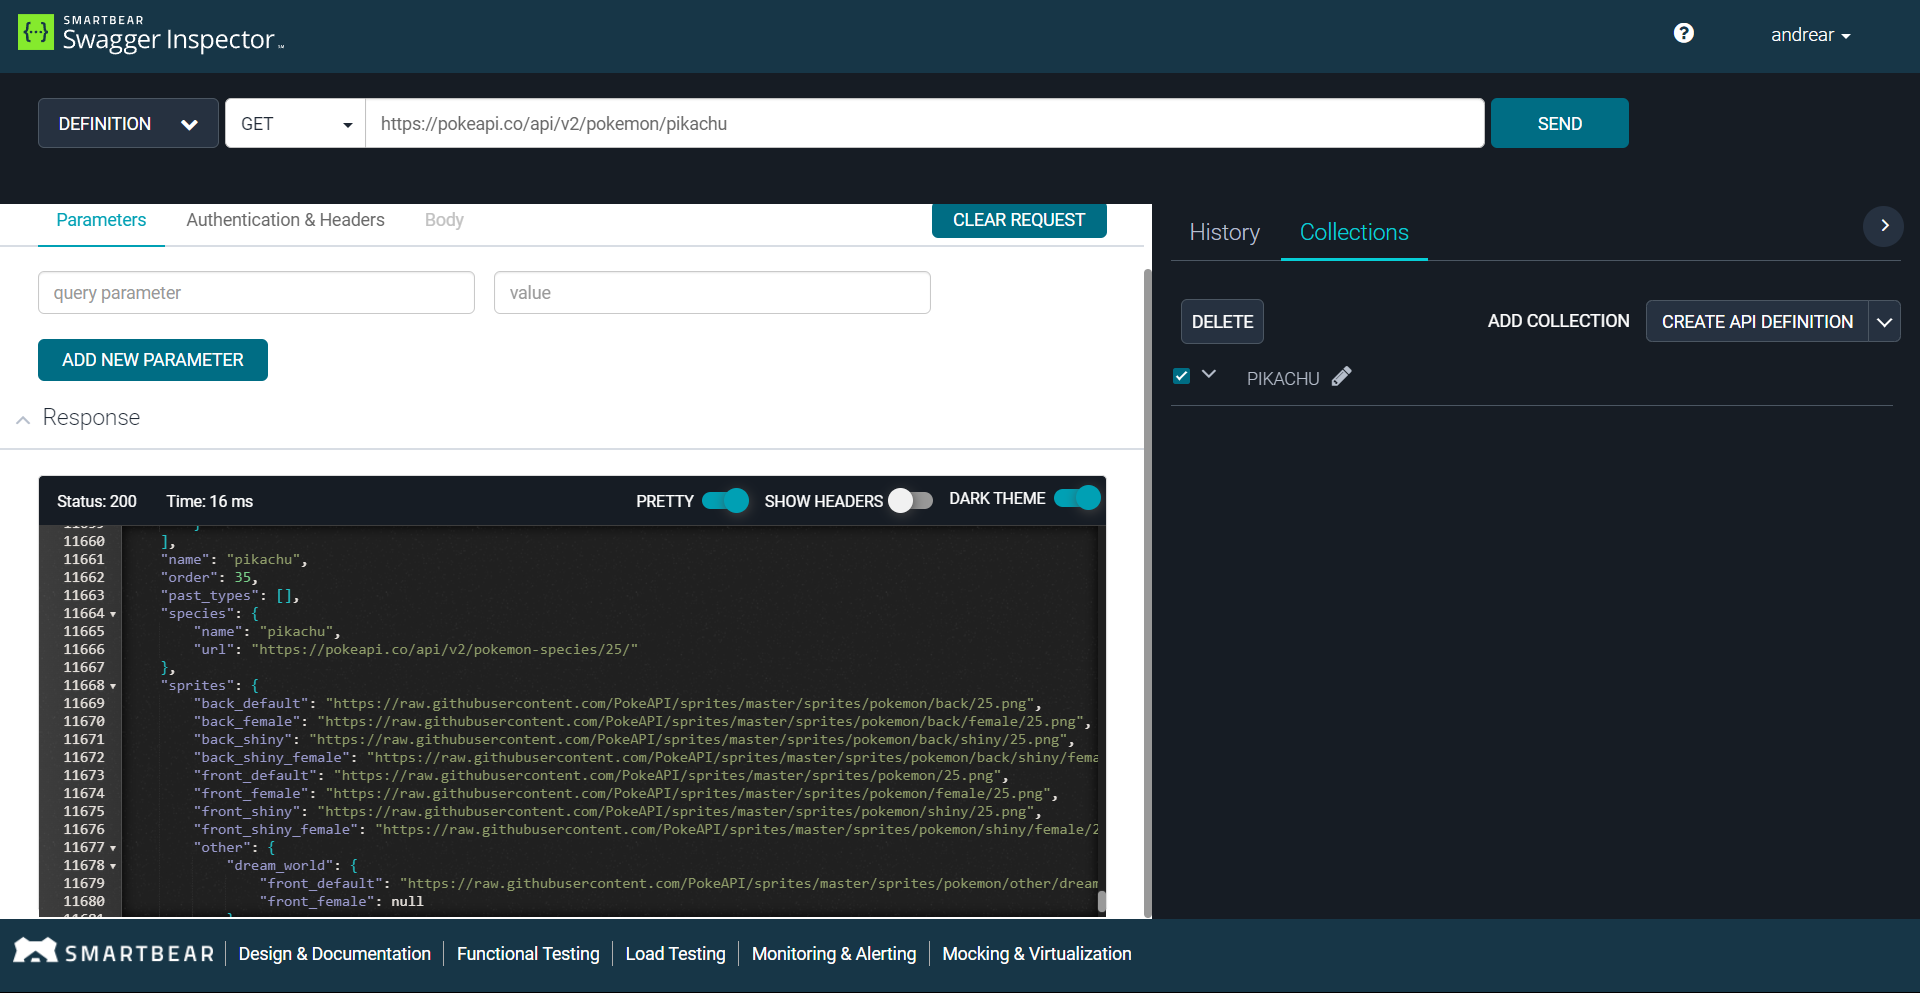
\includegraphics[width=7cm]{./Imagenes/ejemplo1} 
\end{center}
\\ \\

 \textbf{example in Swagger Inspector  }
 \begin{center}
	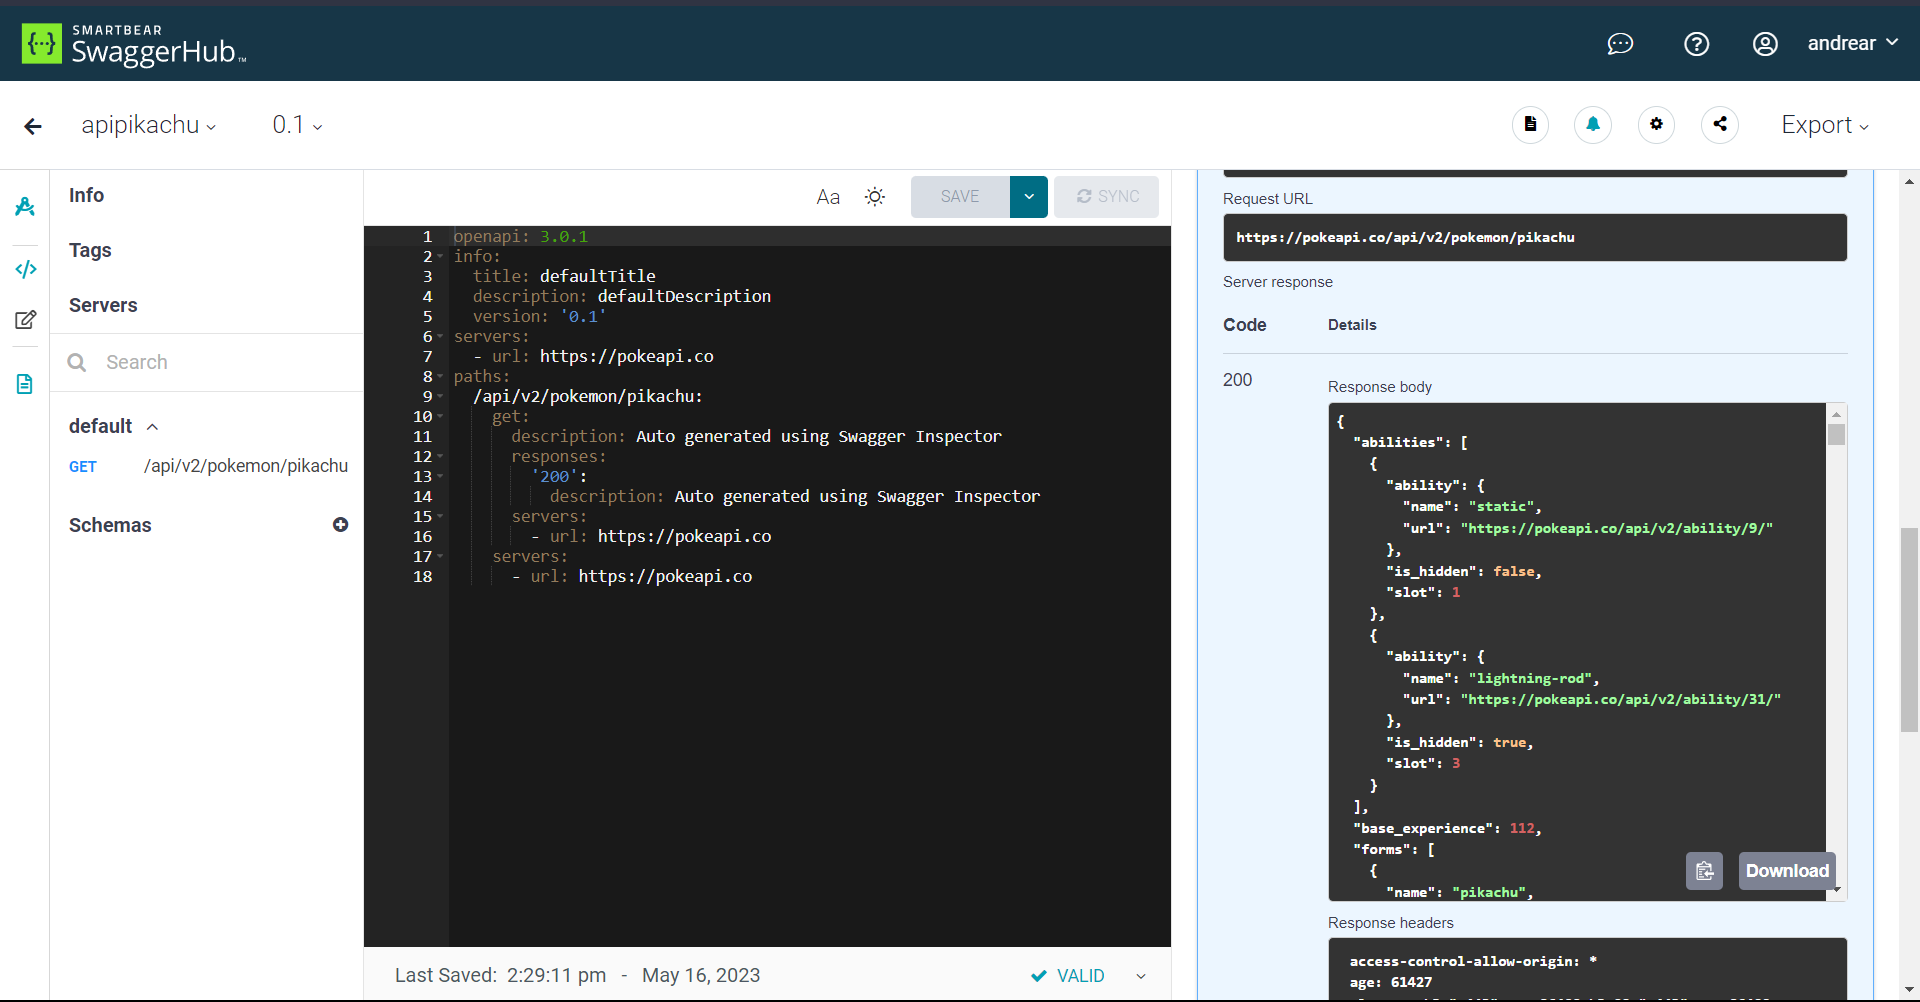
\includegraphics[width=7cm]{./Imagenes/ejemplo2} 
\end{center}
\\ \\


\subsection{Postman}
Postman is a widely-used API development environment that aims to simplify and streamline the process of working with APIs. It provides a user-friendly interface and a range of features designed to support developers at every stage of their workflow. As described by Lane (2015), Postman facilitates tasks such as testing, documentation, and sharing of APIs. With its intuitive interface and robust capabilities, developers can create and manage collections of API requests, organize them into folders, and even automate workflows through tests and scripts. Gartner (2018) highlights that Postman is particularly helpful for automating API testing, enabling developers to easily set up, manage, and run tests for RESTful web services. By offering an environment that enhances productivity and collaboration, Postman has become a go-to tool for developers in the API space.\\\\
 \textbf{characteristics}
\begin{itemize}	
	\item User-Friendly Interface: Postman offers an intuitive and user-friendly interface, making it easy for developers to interact with APIs and perform various tasks.

\item HTTP Request Testing: Postman allows developers to send different types of HTTP requests (such as GET, POST, PUT, DELETE) to APIs and examine the responses. It supports handling parameters, headers, and body content within requests.

\item Collections and Folder Organization: Developers can create and manage collections of API requests in Postman, organizing them into folders for better organization and efficiency.

\item Test Automation: Postman provides capabilities for automating API tests. Developers can add tests and scripts to their collections, allowing for automated testing of endpoints and verification of responses.

\item Collaboration and Sharing: Postman enables collaboration among team members by allowing them to share collections, tests, and documentation. It simplifies the process of sharing and working together on API development.

\item Request History and Versioning: Postman maintains a history of requests made, allowing developers to refer back to previous requests and responses. It also supports versioning of API requests and documentation.

\item Environment Variables: Postman supports the use of environment variables, allowing developers to define variables for different environments (e.g., development, staging, production) and easily switch between them.

\item Authentication and Security: Postman offers various authentication methods to test APIs that require authorization. It supports OAuth, API keys, and other authentication mechanisms for secure API testing.

\item Documentation Generation: Postman allows developers to generate documentation for APIs based on their collections, making it easier to share API specifications and usage instructions.

\item Extensibility: Postman can be extended through the use of plugins and integrations with other tools and frameworks, enhancing its capabilities and integration with existing development workflows.
\end{itemize} 


 \textbf{Ejemplo Get}
\begin{center}
	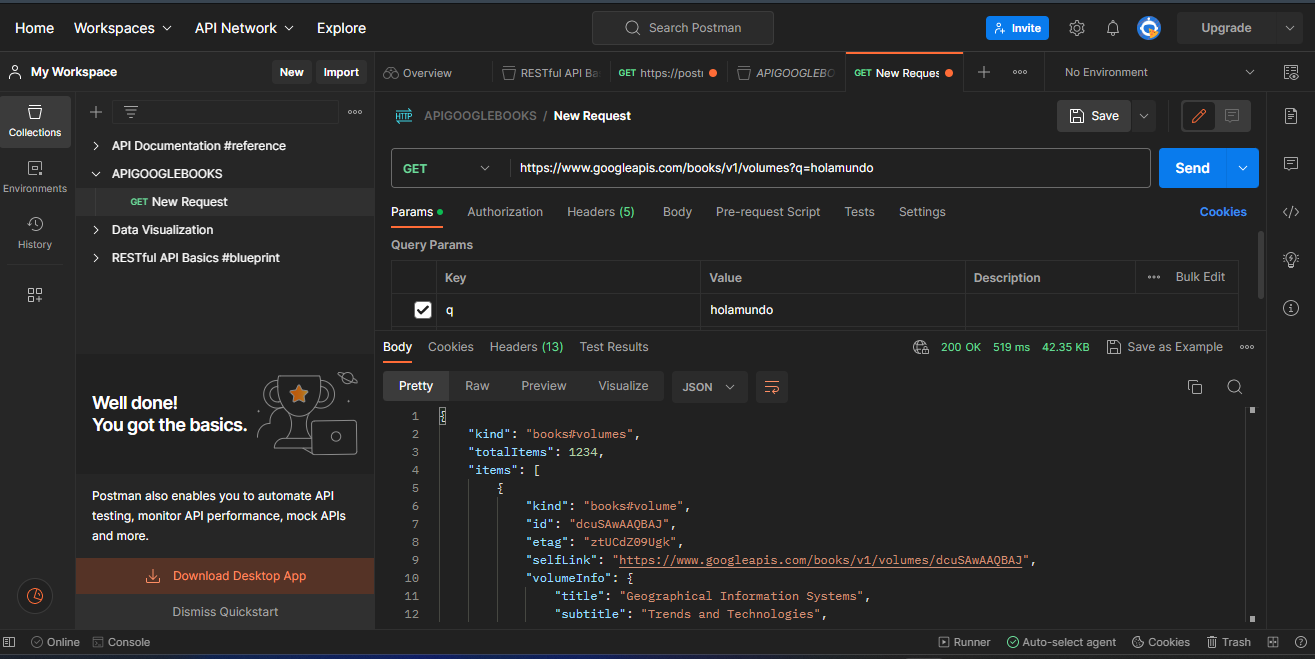
\includegraphics[width=7cm]{./Imagenes/postmanexample} 
\end{center}

\textbf{Ejemplo Get con autorizacion}
\begin{center}
	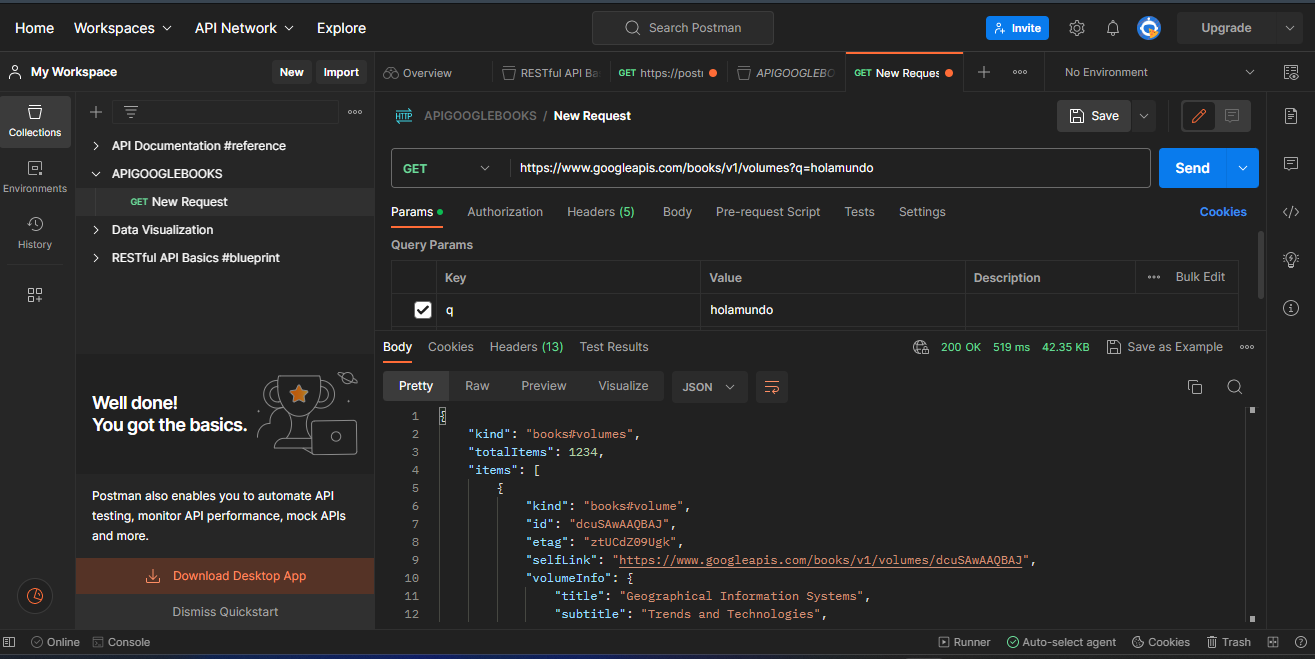
\includegraphics[width=7cm]{./Imagenes/postmanexample} 
\end{center}

 \textbf{Testing and Test Automation}
 
The Testing and Test Automation feature in Postman is one of its key strengths. It provides developers with a comprehensive set of tools and capabilities to perform API testing efficiently. Here's more information about this feature:
\\ \\
Test Creation: Postman allows developers to create tests using a JavaScript-based syntax called "Postman tests." These tests can be added to individual API requests or to entire collections. Developers can write custom tests to validate specific response data, status codes, headers, and more.
\\ \\
Assertion Library: Postman includes a built-in assertion library that offers a wide range of assertion methods. These methods allow developers to define expected values and compare them with actual API responses to determine whether the tests pass or fail. Assertions can be applied to response data, response codes, headers, and other elements.
\\ \\
Test Execution: Once the tests are defined, developers can execute them with a single click. Postman sends the API requests and automatically runs the associated tests, providing instant feedback on the test results. The test results indicate whether the API responses match the expected behavior.
\\ \\
Test Automation: Postman supports test automation, enabling developers to integrate their tests into continuous integration and continuous deployment (CI/CD) workflows. The tests can be executed automatically as part of the build and deployment process, ensuring that APIs function correctly across different environments.
headers, and other elements.
\\ \\
Test Scripts: In addition to tests, Postman allows developers to write pre-request and post-request scripts. Pre-request scripts are executed before sending the API request and can be used, for example, to set up variables or perform data transformations. Post-request scripts run after receiving the API response and can be utilized, for instance, to extract data from the response or perform additional validations.
headers, and other elements.
\\ \\
Test Reporting: Postman provides detailed test reports that summarize the results of test executions. Developers can view these reports within the Postman interface or export them in various formats. Test reports help identify any failures or issues and provide insights into the overall quality and performance of the APIs.
\\ \\
Iterative Testing: Postman allows developers to iterate and refine their tests as they make changes to the API endpoints or the underlying code. The ability to quickly modify and re-run tests helps ensure that APIs remain functional and compliant with the desired specifications.

 \textbf{Collaboration and Teamwork}
  
 The Collaboration and Teamwork feature in Postman is designed to enhance collaboration among team members working on API development projects. It provides a set of functionalities that facilitate communication, sharing, and coordination
 \\ \\
 Workspaces: Postman allows users to create workspaces where teams can collaborate on API-related tasks. Workspaces provide a centralized environment where team members can collectively work on collections, documentation, and other resources.
 \\ \\
Sharing Collections: Within a workspace, users can share collections of API requests with other team members. This allows for easy sharing of API endpoints, headers, parameters, and other relevant information.
 \\ \\
Role-based Access Control: Postman provides role-based access control within workspaces, allowing team administrators to define different levels of access and permissions for team members. This ensures that sensitive information is only accessible to authorized individuals.
 \\ \\
Collaboration Features: Postman offers various collaboration features, such as the ability to leave comments and discussions on specific API requests or collections. Team members can exchange feedback, ideas, and suggestions directly within the Postman interface.
 \\ \\
Version Control: Postman supports version control for collections and other resources, allowing teams to track and manage changes made to APIs over time. It enables better coordination and provides the ability to roll back to previous versions if needed.

\subsection{Comparison between Swagger and Postman}
\begin{itemize}	
	\item  Swagger uses the OpenAPI Specification format for describing and documenting, while Postman does not have a defined language.
	\item Postman has the option of team collaboration by sharing collections, Swagger does not have this option, for this you can use Git.
	\item With Postman you can create automated tests, Swagger is not designed for this.
	\item Swagger focuses on description and documentation, while Postman focuses on API testing.
        \item Postman has an intuitive interface for API testing, Swagger has an intuitive interface for interactive API documentation.
\end{itemize}

\begin{tabular}{| c | c | c |}
\hline
Description & Swagger & Postman \\ \hline
Language & X & -  \\
Interface & X & X  \\
Auto. documentation & X & -  \\
Auto. Tests & - & X  \\

Collaborative work & - & X  \\ \hline
\end{tabular}

%----------------------------------------------------------------------------------------
%	CONCLUSIONES
%----------------------------------------------------------------------------------------

\section{Conclusion}
\begin{itemize}	
	\item  Swagger focuses on API description and documentation, providing a standardized way to define the API structure using the OpenAPI Specification. Swagger UI provides a visual interface for exploring and testing API endpoints, automatically generating useful documentation for understanding and using the API.
	\item Postman focuses on testing and sending HTTP requests to API endpoints. It provides an intuitive interface for creating and organizing requests, and also offers additional features such as automated testing, API monitoring and team collaboration.
	\item Both frameworks are used for testing and documenting APIs, considering that Swagger is strong in documentation and Postman is strong in test automation, deciding which one is better will depend on the specific needs and preferences of the project and team.
\end{itemize} 



\section{Recommendations}
\begin{itemize}	
	\item  Before using an API testing framework, establish clear goals, detailed test cases, and acceptance criteria to guide your efforts and evaluate the results effectively.
	\item Read the documentation of the framework and organize your tests in a structured manner to make the most of its features and facilitate long-term maintenance.
	\item Utilize categories in Postman to separate test cases and share request collections with your team to foster collaboration and knowledge sharing.
	\item Prior to using Swagger or other specification-based tools to generate client code, ensure the validation of the specification to guarantee accuracy and consistency, avoiding issues in the generated code and ensuring reliable results.
\end{itemize} 


%----------------------------------------------------------------------------------------
%	BIBLIOGRAFIA
%----------------------------------------------------------------------------------------


\begin{thebibliography}{99} 

\bibitem[AltexSoft , 2020]{}
\newblock API testing approaches and tools: Postman, rest assured, jmeter, and more, AltexSoft. Available at: https://www.altexsoft.com/blog/api-testing/.

\bibitem[Lane, K. (2015)]{}
\newblock What Is Postman API Development Environment? API Evangelist. 

\bibitem[Gartner, D. (2018)]{}
\newblock  Automating API Testing with Postman. DZone. 

\bibitem[Gesualdo, R. (2021)]{}
\newblock Postman vs. SoapUI: Which is Better for API Testing? BlazeMeter.

\bibitem[Educba. (s.f.)]{}
\newblock Postman vs Swagger Educba. 


\bibitem[Aldaine, A. (2018)]{}
\newblock 10 API testing tools in 2020 

\bibitem[Swagger Inspector. (2021, January 29). Com.Mx. ]{}
\newbloc Revisión de herramientas

\bibitem[IONOS Digital Guide. Retrieved(2023)]{}
\newbloc Swagger más comodidad en el desarrollo de API. (n.d.).
\end{thebibliography}


%----------------------------------------------------------------------------------------


\end{document}
